\documentclass[conference,final]{IEEEtran}

\usepackage{amssymb}
\usepackage{amsmath}

%\usepackage{fullpage}
\usepackage{color}
\usepackage{float}
\usepackage{graphicx}
\usepackage{pgfplots}
\pgfplotsset{%
    compat=newest,
    cycle list={mark=triangle,color=red!75!black\\
                mark=square,color=green!75!black\\
                mark=|,color=white\\
                mark=o,color=blue\\
                mark=pentagon,color=purple\\
                mark=x,color=yellow!50!orange\\
                mark=x,color=brown!75!black\\
                mark=x,color=black!50!white\\},
    every axis plot post/.append style={thick},
    ignore legend/.style={every axis legend/.code={\renewcommand\addlegendentry[2][]{}}}
    }
\usepackage{booktabs}
\usepackage{paralist}

\usepackage{url}
\usepackage{xspace}
\usepackage[utf8]{inputenc}
\usepackage[T1]{fontenc}
\usepackage[english]{babel}
\usepackage[babel]{csquotes}

%%%% Use this to locally disable comments %%%%%
%\usepackage[disable]{todonotes}
\usepackage{todonotes}

\usepackage[binary-units=true]{siunitx}

% fix some latex functions
\usepackage{fixltx2e}

% copyright notice (IEEE)
\usepackage{eso-pic}
\AddToShipoutPicture*{\small\sffamily\raisebox{1.8cm}{\hspace{1.8cm}978-1-4799-5944-0/14/\$31.00
 \copyright2014 IEEE}} 

\usepackage[ruled,linesnumbered,algosection,algo2e]{algorithm2e}
\SetAlFnt{\small}
\SetAlCapFnt{\small}
\SetAlCapNameFnt{\small}

% fix for two column algorithms
\makeatletter
\newcommand{\removelatexerror}{\let\@latex@error\@gobble}
\makeatother

% correct spacing for et al., i.e. and e.g.
\newcommand{\ie}{\text{i.\,e., }}
\newcommand{\eg}{\text{e.\,g., }}
\newcommand{\detal}{\textit{et~al.}}
\newcommand{\cf}{\text{cf. }}

\usepackage{hyperref}

%%%%%%%%%%%%%%%%%%%%%%%%%%%%%%%
% Macros for ToDos etc.
% Feel free to add you name as well...
%%%%%%%%%%%%%%%%%%%%%%%%%%%%%%%%
\newcommand{\itodo}[1]{
  \todo[inline]{#1}
}
\newcommand{\inote}[2]{
  \itodo{#1: #2}
}
\newcommand\RZ[1]{\inote{RZ}{{#1}}}
\newcommand\FW[1]{\inote{FW}{{#1}}}

\begin{document}
\title{High-Speed Implementation of bcrypt Password Search using Special-Purpose
Hardware}

\author {
\IEEEauthorblockN{
    Friedrich Wiemer,
    Ralf Zimmermann
    }
\IEEEauthorblockA{
    Horst G\"ortz Institute for IT-Security (HGI), Ruhr-University Bochum,
	Germany \\
	Email: {\tt\{friedrich.wiemer, ralf.zimmermann\}@rub.de}
  }
}

\maketitle

%!TEX root = main.tex

\begin{abstract}
Using passwords for user authentication is still the most common method for many
internet services and attacks on the password databases pose a severe threat. To
reduce this risk, servers store password hashes, which were generated using
special password-hashing functions, to slow down guessing attacks. The most
frequently used functions of this type are PBKDF2, bcrypt and scrypt.\\
%
In this paper, we present a novel, flexible, high-speed implementation of a
bcrypt password search system on a low-power Xilinx Zynq 7020 FPGA. The design
consists of 40 parallel bcrypt cores running at 100 MHz. Our implementation
outperforms all currently available implementations and improves password
attacks on the same platform by at least 42\%, computing 6,511 passwords per
second for a cost parameter of 5.
%
%We compare our results to other platforms, \ie CPUs, GPUs and a Xilinx Virtex-7
%FPGA, and evaluate the total cost for multiple attacking scenarios using the
%different platforms and implementations.
\end{abstract}

\section{Introduction}
\label{sec:intro}

In the modern world, we constantly use online services in our daily life. As a
consequence, we provide information to the corresponding service providers,
\eg financial services, email providers or social networks. To prevent abuse
like identity theft, we encounter access-control mechanisms at every step we
make. While it is one of the older mechanisms, password authentication is still
one of the most frequently used authentication methods on the internet even
with the emerging advanced login-procedures, \eg single sign-on or two-factor
authentications.
% passwords remain a necessary part.

To authenticate users for online services, these passwords are stored on
corresponding servers. As a consequence, an attack on these databases, followed
by a leak of the information, pose a very high threat to the users and may form
a single point of failure, if the passwords are stored in plain text. Recent
examples of such leaks are the eBay\footnote{\cf
\url{http://www.ebayinc.com/in_the_news/story/ebay-inc-ask-ebay-users-change-
passwords}} or Adobe\footnote{\cf \url{https://adobe.cynic.al/}} password leaks,
where several million passwords were stolen. To prevent these attacks or at
least raise the barrier of abuse, passwords must be protected on the server.
Instead of storing the password as plaint text, a cryptographic hash of the
password is kept. In this case, a successful attacker has to recover the
passwords from the hash value, which should in theory be infeasible due to the
properties of the hash function. To prevent time-memory trade-off techniques
like rainbow tables, the password is combined with a randomly chosen salt and
the tuple
\begin{equation*}
	(s, h) = (salt, \text{hash}(salt, password))
\end{equation*}
is stored. Improvements to exhaustive password searches with the aim to
determine weak passwords exists. As passwords are often generated from a
specific character set, \eg using digits, upper- and lower-case characters, and
may be length-restricted, \eg allowing six to eight characters, the search space
can be reduced considerably. This enables password recovery by brute-force or
dictionary attacks. Recently, more advanced methods,
\eg probabilistic context-free grammars~\cite{PWDCrackGrammars} or Markov
models~\cite{FastDictAttacks,OMEN} were analyzed to improve the password guesses
and the success rate and thus reduce the number of necessary guesses.

Apart from the generation of suitable password candidates, the implementation has a
high impact on the success. On general-purpose CPUs, generic tools like
\emph{John the Ripper} (JtR)\footnote{cf. \url{http://www.openwall.com/john}} or
target-specific tools like \emph{TrueCrack}\footnote{cf.
\url{http://code.google.com/p/truecrack}}, addressing a specific algorithm, in
this case TrueCrypt volumes, use algorithmic optimizations to gain a speedup
when testing multiple passwords. To further improve efficiency, not only the CPU
may be used: modern GPUs feature a large amount of parallel processing cores at
high clock-frequencies in combination with large memory. As a prominent example,
\emph{HashCat}\footnote{cf. \url{http://hashcat.net/oclhashcat}} utilizes this
platform for high-performance hash computations.

The major problem remains that hash functions are very fast to evaluate and thus
enable fast attacks. \emph{Password-hashing functions} address this issue. These
functions map a password to key material for further usage and explicitly slow
down the computation time by making heavy use of the available resources: the
computation should be fast enough to validate an honest user, but render
password guessing infeasible. One key idea to prevent future improvements in
architectures from breaking the efficiency of these function are flexible cost
parameters. These adjust the function in terms of time and/or memory complexity.

The current standardized password-based key-derivation function is PBKDF2 which
is part of the Public-Key Cryptography Standards (PKCS)~\cite{RFC2898}.
Non-standardized alternatives are bcrypt~\cite{BCRYPT_paper} and
scrypt~\cite{percival-09-scrypt}.
%Both are frequently used and feature different security approaches, \eg
%requiring very large memory or frequently accessing small memory randomly.
While the three functions are considered secure, each has its own advantages
and disadvantages. This lead to the currently running password hashing
competition (PHC)\footnote{\cf \url{https://password-hashing.net/}}, which aims
at providing well-analyzed alternatives. Another purpose is discussing new ideas
and different security models with respect to the impact of special-purpose
hardware like modern GPUs, Application-Specific Integrated Circuits
(ASICs) or Field-Programmable Gate Arrays (\mbox{FPGAs}).

Usually, the overall cost of large-scale attacks on cryptographic functions --
and thus the feasibility of the attack -- is dominated by the power costs. For
this reason, specialized hardware achieves excellent results due to its low
power consumption, especially when compared to general-purpose architectures.
This makes special-purpose hardware very attractive for cryptanalysis in
general~\cite{CryptanalysisCOPA, EnhancingCOPA, RealWorldA51, FPGAFactoring},
as well as in the context of password-hashing functions~\cite{PBKDEvalutation}.

For the remainder of this paper, we focus on bcrypt as the target function in
the scope of efficient password-guessing attacks and start with an overview on
the currently available implementations. In Section~\ref{sec:bcrypt}, we describe the bcrypt
algorithm and the influence its tunable cost parameter.

With the goal of benchmarking energy-efficient password cracking,
\cite{PWDCON_Bcrypt} provided several implementations of bcrypt on low-power
devices, including an FPGA implementation in December 2013. The authors used the
zedboard (cf. \ref{sec:special-hardware}), which combines an ARM processor and
an FPGA, and split the workload on both platforms. The FPGA computes the
time-consuming cost-loop of the algorithm while the ARM manages the setup and
post-processing. They reported up to 780 passwords per second (pps) for a cost
parameter of 5 and identified the highly unbalanced resource usage as a drawback
of the design.
%
In August 2014, \cite{WOOT/Malvoni14} presented
%\footnote{The article was
%accepted at WOOT'14 and will be presented on August 19, 2014. We were notified
%about the results and provided with information about the content of the final
%version. This paragraph and the numbers may be updated once the paper and
%presentation are public.}
a new design, improving the performance to 4571 pps
for the same device and parameter, using the ARM only for JtR to generate
candidates and to transfer initialization values to the FPGA. When they further
optimized performance, the zedboard became unstable (heat and voltage problems).
Due to these issues they also report a higher theoretical performance of 8122
pps (derived from cost 12) and 7044 pps (simulated using the larger Zynq 7045
FPGA).

\emph{Contribution:} In this paper, we provide a practical and efficient
implementation of bcrypt on a low-power FPGA-platform. Compared to the previous
implementations on the same device, we achieve a performance gain of 8.35 and
1.42, respectively.
%, and outperform the theoretical upper bounds by more than 60\%.
In addition, we implemented a simple on-chip password generation to
utilize free area in the fabric, which splits a pre-defined password space and
generates all possible brute-force candidates. This creates a self-contained,
fully functional system (which may still use other sources for password
candidate checking), which we compare to other currently available
attack-platforms.

\emph{Outline:} The rest of the paper is structured as follows: We first
introduce the necessary background information in Section~\ref{sec:background},
before we describe our implementation details in the subsequent section and
discuss our results, followed by an evaluation of the costs of different attack
scenarios, in Section~\ref{sec:results}. Finally, our conclusion and
perspectives for future work form the last section.

%!TEX root = main.tex

\section{Background}
\label{sec:background}

In this section, we introduce the bcrypt algorithm and outline the
computationally expensive steps to motivate the design decisions we made. The
second part gives a short overview of our two target FPGA families and their
features.

\subsection{The bcrypt password hash}
\label{sec:bcrypt}


Provos and Mazi\`{e}res published the bcrypt hash function~\cite{BCRYPT_paper}
in 1999, which, at its core, is a cost-parameterized, modified version of the
Blowfish encryption algorithm. The key concepts are a tunable cost parameter and
the pseudo-random access of a 4 KByte memory. bcrypt is used as the default
password hash in OpenBSD since version 2.1~\cite{BCRYPT_paper}. Additionally, it
is the default password hash in current versions of Ruby on Rails and PHP.

\begin{figure*}[tb] \centering
\removelatexerror
\begin{minipage}{.45\linewidth}
\begin{algorithm2e}[H]
	\KwIn{cost, salt, key}
	\KwOut{state}
	$state \leftarrow$ InitState$()$\;
	$state \leftarrow$ ExpandKey$(state, salt, key)$\;
	\KwSty{Repeat} ($2^{cost}$) \Begin{
		$state \leftarrow$ ExpandKey$(state, 0, salt)$\;
		$state \leftarrow$ ExpandKey$(state, 0, key)$\;
	}
	\KwRet{$state$}\;
	\caption{EksBlowfishSetup}
	\label{alg:eksblowfishsetup}
\end{algorithm2e}
\end{minipage}
	\hspace{0.5cm}
\begin{minipage}{.45\linewidth}
\begin{algorithm2e}[H]
	\KwIn{cost, salt, key}
	\KwOut{hash}
	$state \leftarrow$ EksBlowfishSetup$(cost,salt,key)$\;
	$ctext \leftarrow$ ``OrpheanBeholderScryDoubt''\;
	\KwSty{Repeat} ($64$) \Begin{
		$ctext \leftarrow$ EncryptECB$(state, ctext)$\;
	}
	\KwRet{Concatenate$(cost,salt,key)$}\;
	\caption{bcrypt}
	\label{alg:bcrypt}
\end{algorithm2e}
\end{minipage}
\end{figure*}

bcrypt uses the parameters \textit{cost}, \textit{salt}, and \textit{key} as
input. The number of executed loop iterations is exponential in the
\textit{cost} parameter, \cf Algorithm~\ref{alg:eksblowfishsetup}
(\texttt{EksBlowfishSetup}). The computation is divided into two phases: First,
Algorithm~\ref{alg:eksblowfishsetup} initializes the internal state, which has
the highest impact on the total runtime. Afterwards, Algorithm~\ref{alg:bcrypt}
(\texttt{bcrypt}) encrypts a fixed value repeatedly using this state.


In its structure, bcrypt makes heavy use of the Blowfish encryption function.
This is a standard 16-round Feistel network, which uses SBoxes and subkeys
determinded by the current $state$. Its blocksize is 64-bit and during every
round, an f-function is evaluated: it uses the 32-bit input as four 8-bit
addresses for the SBoxes and computes $(S_0(a) + S_1(b)) \oplus S_2(c) + S_3(d)$
%
\texttt{EksBlowfishSetup} is a modified version of the Blowfish key schedule. It
computes a state, which consists of 18 32-bit subkeys and four SBoxes -- each
256 $\times$ 32 bits in size -- which are later used in the encryption process.
The state is initially filled with the digits of $\pi$ before an
\texttt{ExpandKey} step is performed: After adding the input key to the subkeys,
this step successively uses the current state to encrypt blocks of its
\textit{salt} parameter and updates it with the resulting ciphertext. In this
process, \texttt{ExpandKey} computes 521 Blowfish encryptions. If the salt is
fixed to zero, the function resembles the standard Blowfish key schedule. An
important detail is that the input key is only used during the very first part
of the \texttt{ExpandKey} steps. \texttt{bcrypt} finally uses
\texttt{EncryptECB}, which is effectively a Blowfish encryption.

\subsection{Special-Purpose Hardware}
\label{sec:special-hardware}

While general-purpose hardware, \ie CPUs, offers a wide variety of instructions
for all kinds of programs and algorithms, usually only a smaller subset is
important for a specific task. More importantly, the generic structure and
design of the architecture might impose restrictions and become cumbersome, \ie
when registers are too small or memory access latency becomes a bottleneck.
Reconfigurable hardware like FPGAs and special-purpose hardware like ASICs are
far more specialized -- they are dedicated to a single task.

An FPGA consists of a large area of programmable logic resources (the fabric),
\eg lookup tables (LUTs), shift registers, multiplexers and storage elements,
and a fixed amount of dedicated hardware modules, \eg memory cores (BRAM),
digital signal processing units or even processor hardcores, and can be
specialized for a given task.
%
In this work, we target two different Xilinx FPGA families. The main platform is
zedboard, more precisely its Zynq-7000 XC7Z020 FPGA. It is located in the
low-power low-cost segment. The second target is the Virtex-7 XC7VX485T FPGA
which is a high-performance device.

The Zynq-7000 consists mainly of a dual-core ARM Cortex A9 CPU, while the fabric
area and resources are comparable to an Xilinx Artix-7 FPGA. The zedboard allows
easy access to the logic inside the fabric and memory modules via direct memory
access and provides several interfaces, \eg AXI4, AXI4-Stream, AXI4-Lite or
Xillybus. It is a good choice for hardware/software co-design and in the context
of this work provides a self-contained system including complex means for
password generation and fast hardware designs. The Virtex-7 on the other hand,
offers a five times larger fabric area and seven times more memory cores at the
cost of more power consumption and a higher device price.

%!TEX root = main.tex

\section{Implementing bcrypt on FPGAs}
\label{sec:implementation}

In this section, we describe our FPGA implementation of a multi-core bcrypt
cracker, capable of both on-chip password generation and offline dictionary
attacks. We start with the general design decisions, the results of an early
version of our design and discuss the choices we made to improve the overall
design.

An efficient implementation should result in a balanced usage of the available
dedicated hardware and fabric resources and maximize the number of parallel
instances on the device. In the case of bcrypt, using one dual-port BRAM
resource to store two SBoxes saves LUT resources, results in high clock
frequencies and relaxes the routing without creating wait-states. To increase
the utilization of the memory, we focused on shared memory access without adding
clock cycles to the main computation. In the final design, one bcrypt core
occupies three BRAM blocks with two additional global memory resources for the
initialization values. This leads to an upper bound of 46 cores per zedboard
(ignoring any extra BRAM usage of the interface).

Considering a brute-force attack to benchmark the capabilities of the FPGA, the
interface can be minimalistic. We use a bussystem with minimal bandwidth
capacity, resulting in a small on-chip area footprint. For this scenario, we
chose the following setup: During start-up, the host transfers a 128-bit target
salt and a 192-bit target hash to the FPGA. These values are kept in two
registers to allow access during whole computation time. After filling the
registers, all bcrypt cores start to work in parallel. The password candidates
are generated on-chip. When the attack completes, a successful candidate is
transferred back to the host.

Our earlier design was built out of fully independent bcrypt cores. Each core
contained its own password register as well as the memory for the initialization
values. This effectively removed all cross-dependencies and resulted in very
short routing delays and thus very high clock frequencies. Due to Blowfish's
simple Feistel structure, only a small amount of combinatoric logic was needed:
Since the main work is done via BRAM lookups. Nevertheless, storing the password
in fabric consumes far too much area and resulted in an unbalanced
implementation. However, the timing results indicated that more than 100 MHz
should be possible.

\begin{figure}[tp] \centering
	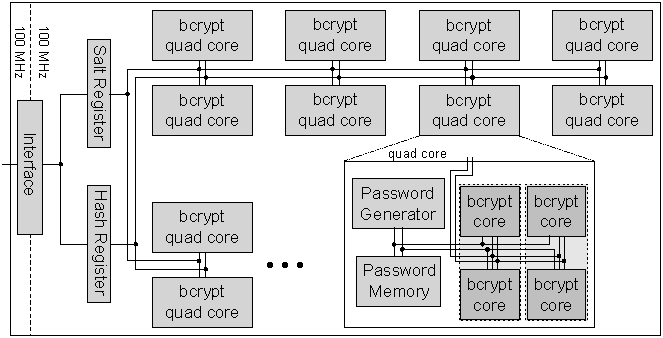
\includegraphics[width=0.475\textwidth]{figures/bcrypt_design_overview.pdf}
	\caption{Schematic Top-Level view of FPGA implementation. The design
	uses multiple clock-domains: a (slow) interface clock and a fast bcrypt
	clock. Each quad-core accesses the salt- and hash registers and consists of 
	a dedicated password memory, four bcrypt cores and a password generator.}
	\label{fig:bcrypt_design_overview}
\end{figure}

In order to reduce the area footprint, we tried to share resources and
analyzed the algorithm for registers that are not constantly accessed by all
cores. We first removed the initialization memory and used the free register
resources to implement a pipeline and buffer the signals such that the critical
path was unaffected by the change. Due to the required memory access and the
dual port properties, we also combined four bcrypt cores with one password
generator and password memory. These \emph{quad-cores} can schedule password
accesses with negligible overhead.

\begin{figure*}[tp] \centering
	\begin{minipage}[b]{0.45\textwidth} \centering
		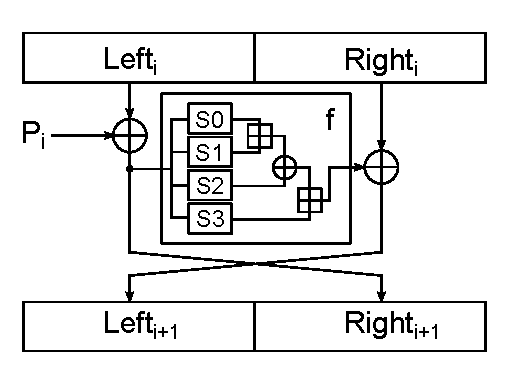
\includegraphics[height=3.5cm]{figures/blowfish_feistel.pdf}
		\caption{The normal Feistel-structure of one standard Blowfish round.
		         Note that the final XOR operation may be moved along the datapath.
				 By delaying it to the next round, we can resolve data
				 dependencies and compute one Blowfish round in one clock
				 cycle more efficiently.}
		\label{fig:blowfish-feistel}
	\end{minipage}%
	\hspace{0.5cm}
	\begin{minipage}[b]{0.45\textwidth} \centering
		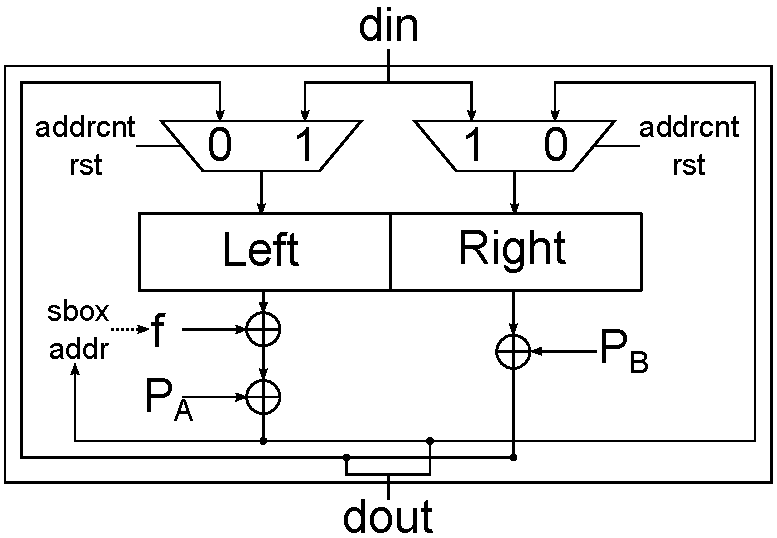
\includegraphics[height=3.5cm]{figures/blowfish_core.pdf}
		\caption{Blockdiagram of Blowfish core. The computation of the delayed 
                 f-function is integrated into the left half and the result of
				 the modified data-path forms the memory address for the next f-function.}
		\label{fig:blowfish-core}
	\end{minipage}
\end{figure*}

These changes reduced the area consumption by roughly 20\% at the cost of one
additional BRAM resource per quad-core. Figure~\ref{fig:bcrypt_design_overview}
shows the resulting design using multiple parallel and independent quad-cores.
Every bcrypt core starts its operation with the initialization of the 256 SBox
entries. Within this timeslot, the password generator produces four new
passwords and writes them into the password memory. By using the dual-port
structure of the memory, two bcrypt cores access their passwords in parallel.
While these first two cores uses the BRAM, the second pair of cores is stalled.
This leads to a delay of 19 clock cycles between both pairs.

The bcrypt core spents most of the time within Blowfish encryptions, as these
are used during the \texttt{ExpandKey} (521 times) and \texttt{EncryptECB} (3
times) steps. Thus, optimizing the Blowfish core heavily improves the overall
performance. A na\"ive implementation needs two clock cycles per Blowfish round:
one to calculate the input of the f-function -- and thus the addresses to the
SBox entries -- and one to compute the XOR operation on the f-function output
and the subkey.

Figure~\ref{fig:blowfish-feistel} shows the standard Blowfish Feistel round. We
moved the XORs along the datapath, changing the round boundaries. This delay
allows us to prefetch the subkeys from the memory and resolve data-access
dependencies to reduce the cycle count to one per round.

The resulting Blowfish core is depicted in Figure~\ref{fig:blowfish-core}. All
of the three XOR operations -- the f-function's output and the subkeys
$\text{P}_\text{A}$ and $\text{P}_\text{B}$ -- are computed in every round,
removing all multiplexers from the design. As this would change the Blowfish
algorithm, we use the reset of the BRAM output registers to suppress any invalid
XOR operations during the computation. This design leads to a very minimalistic
control logic and a very small Blowfish design in terms of area. Concerning the
critical path, the maximum delay comes from the path from the SBox through the
evaluation of the f-function.
%\footnote{To address this problem, we designed a
%pipelined, interleaved Blowfish module, which all four cores of the quad-core
%share. These results are still pending and will be included later, if the
%paper is accepted and the addition is allowed.}

We have roughly a fourth of the available slices left when we reach the limit of
available memory blocks. These resources can be utilized for the password
generation. In its simplest form, this is very efficient on-chip, as it only
requires a small amount of logical resources.
%Figure~\ref{fig:password_generation} provides a schematic overview.
For each  password byte, one counter and register store the current states. The
initialization value differs for every core and determines the search space. The
logic always generates two subsequent passwords and enumerates over all possible
combinations for a given character set and maximum password length. When the
state has been updated correctly, it is mapped into ASCII representation and
written into the password memory. The generation process finishes during the 256
initialization clock cycles, leaving enough time to buffer the signals and
ensure a low amount of levels-of-logic.

%\begin{figure}[tp] \centering
%	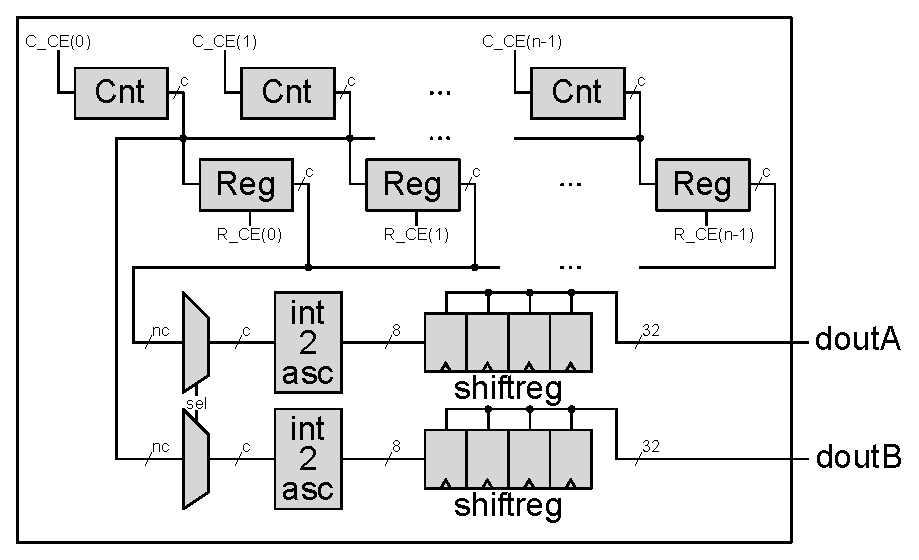
\includegraphics[width=0.475\textwidth]{figures/password_gen.pdf}
%	\caption{Schematic view of the password generation. The counter and registers in
%	the upper half store the actual state of the generator. The mapping to ASCII
%	characters is done by multiplexer. It uses a cyclic output for bcrypt and
%	generates two passwords in parallel.}
%	\label{fig:password_generation}
%\end{figure}

Please note that with this design, even a slow and simple interface capable of
sending 320 bits and a start flag can use the system for brute-force attacks.
A more complex interface -- capable of fast data-transfer or even direct memory
access of the BRAM cores -- easily enables dictionary attacks, as new
passwords are transferred directly into the password memory during the long
bcrypt computation. The on-chip password generation may be removed or modified
to work in a hybrid mode.

%!TEX root = main.tex

\section{Results}
\label{sec:results}

\begin{table*}[tp] \centering
	\begin{minipage}[b]{0.35\textwidth} \centering
		\caption{Resource utilization of design and submodules.}
		\label{tab:results_resource_utilization}
		\begin{tabular}{l r r r r}
			\toprule
							   &    LUT    &    FF     &   Slice   &   BRAM    \\
			\midrule
			Overall            &  64.8\% & 13.06\% & 93.29\% & 95.71\% \\
			\midrule
			quad-core          &  2,777  &    720  &    801  &   13    \\
			single core        &    617  &    132  &    197  &    3    \\
			Blowfish core      &    354  &     64  &     71  &    0    \\
			Password Generator &    216  &    205  &     81  &    0    \\
			\bottomrule\\
		\end{tabular}
	\end{minipage}%
	\hspace{1.5cm}
	\begin{minipage}[b]{0.5\textwidth} \centering
		\caption{Comparison of multiple implementations and platforms, considering
		full system power consumption.}
		\label{tab:results_different_plattforms}
		\begin{tabular}{l c c c c c c}
			\toprule
			& \multicolumn{2}{c}{cost parameter 5}
			& \multicolumn{2}{c}{cost parameter 12}
			& & \\
			& $\frac{\text{Hashes}}{\text{Second}}$
			& $\frac{\text{Hashes}}{\text{Watt Second}}$
			& $\frac{\text{Hashes}}{\text{Second}}$
			& $\frac{\text{Hashes}}{\text{Watt Second}}$
			& Power & Price \\
			\midrule
			zedboard     &  6,511 & 1,550 &  51.95 & 12.37 & \SI{4.2}{\watt} &   \$319 \\
			Virtex-7     & 51,437 & 2,572 & 410.4  & 20.52 & \SI{ 20}{\watt} & \$3,495 \\
			\midrule
			Xeon E3-1240 &  6,210 &  20.7 &  50    &  0.17 & \SI{300}{\watt} &   \$262 \\
			GTX 750 Ti   &  1,920 &   6.4 &  15    &  0.05 & \SI{300}{\watt} &   \$120 \\
			\midrule
			\cite{WOOT/Malvoni14}~Epiphany 16 &  1,207 & 132.64 &  9.64 & 1.06 & \SI{9.1}{\watt} &   \$149 \\
			\cite{WOOT/Malvoni14}~zedboard    &  4,571 & 682.24 & 64.83 & 9.68 & \SI{6.7}{\watt} &   \$319 \\
			\bottomrule\\
		\end{tabular}
	\end{minipage}%
\end{table*}

In this section we will present the results of our implementation. We used
Xilinx ISE 14.7 and -- if needed Xilinx Vivado 2014.1 -- during the design flow
and verified the design both in simulation and on the zedboard after Place and
Route.

Table~\ref{tab:results_resource_utilization} provides the post place-and-route
results of the full design on the zedboard. We implemented the design using ten
parallel bcrypt quad-cores and a Xillybus interface. The design achieves a clock
frequency of 100 MHz. The optimizations from Section~\ref{sec:implementation}
reduced the LUT consumption to roughly 600 LUTs, the amount of BRAMs to 3.25
per single core. We therefore can fit ten quad-cores -- and thus 40 single cores
-- on a zedboard, including the on-chip password generation.

The bcrypt cores need constant cycles $c$ for hash generation, in detail:
\begin{equation*}
\begin{aligned}[c]
c_\text{Reset} &= 1\\
c_\text{Delay} &= 19\\
c_\text{bf} &= 18\\
c_\text{key xor} &= 19\\
\end{aligned}
%\quad
%\begin{aligned}[c]
%\end{aligned}
\quad
\begin{aligned}[c]
c_\text{Init} &= 256\\
c_\text{Pipeline} &= n,\, (n = 2)\\
c_\text{updateP} &= 9 \cdot (c_\text{bf})\\
c_\text{updateSBox} &= 512 \cdot (c_\text{bf})\\
\end{aligned}
\end{equation*}
\begin{align*}
c_\text{ExpandKey} &= c_\text{key xor} + c_\text{upP} + c_\text{upSBox} = 9,397\\
c_\text{EncryptECB} &= 3 \cdot 64 \cdot (c_\text{bf} - 1) = 3,264
\end{align*}
Following these values, one bcrypt hashing needs
\begin{align*}
c_\text{bcrypt} &= c_\text{Reset} + c_\text{Pipeline} + c_\text{Init} +
				   c_\text{Delay} +\\
				&\quad (1 + 2^{\text{cost}+1} \cdot c_\text{ExpandKey}) +
				   c_\text{EncryptECB}\\
				&= 12,939 + 2^{\text{cost}+1} \cdot 9,397
\end{align*}
cycles to finish. This leads to a total of 614,347 cycles per password (cost
5) and 76,993,163 (cost 12), respectively.

In order to compare the design with other architectures, especially with the
previous results on the zedboard, we measured the power consumption of the board
during a running attack and used (ocl)Hashcat to benchmark a Xeon E3-1240 CPU (4
cores@3.1 GHz) and a GTX 750 Ti (Maxwell architecture) as representatives for
the classes of CPUs and GPUs. Furthermore, we synthesized our quad-core
architecture on the Virtex 7 XC7VX485T FPGA, which is available on the VC707
development board, and estimated the number of available cores with respect to
the area a new interface may occupy. We assume a worst-case upper bound of 20W
as the power consumption for the full evaluation board.
For the CPU and the GPU attack, we also consider the complete system. While
there are smaller power supplies available, we consider a 300W power supply,
which is the recommended minimum for the GPU to run stable.

\begin{figure}[tp]
	\centering
	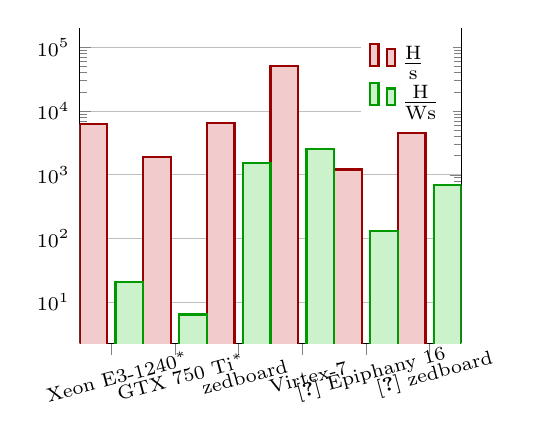
\begin{tikzpicture}[color/.style={draw=#1!80!black,fill=#1!20}]
	\pgfplotsset{
		height=4cm, width=.4\textwidth,
		scale only axis,
		legend style={draw=none,legend cell align=left}}
	\begin{axis}[
		axis x line*=bottom,
		x tick label style={rotate=15,anchor=south,yshift=-5mm,font=\scriptsize},
		y tick label style={font=\scriptsize},
		xtick={1, 2, 3, 4, 5, 6},
		xticklabels={
			Xeon E3-1240$^*$,
			GTX 750 Ti$^*$,
			zedboard,
			Virtex-7,
			\cite{WOOT/Malvoni14}~Epiphany 16,
			\cite{WOOT/Malvoni14}~zedboard},
		xmin=0.5, xmax=6.5,
		ymin=0, ymax=200000,
		ymode=log,
		ymajorgrids=true,
		ybar=3pt,
		bar width=10pt,
		]
		\addplot+[color=red!75!black] plot coordinates{
			(1, 6210)
			(2, 1920)
			(3, 6511)
			(4, 51437)
			(5, 1207)
			(6, 4571)};
		\addplot+[color=green!75!black] plot coordinates{
			(1, 20.7)
			(2, 6.4)
			(3, 1550)
			(4, 2572)
			(5, 132.64)
			(6, 682.24)};
		\legend{$\frac{\text{H}}{\text{s}}$,$\frac{\text{H}}{\text{Ws}}$}
	\end{axis}
	\end{tikzpicture}
	\caption{Comparison of different implementations for cost parameter 5. Left bars
	(red) show the hashes-per-seconds rate, right bars (green) the
	hashes-per-watt-seconds rate. Results with $^*$ were measured with
	(ocl)Hashcat. The axial scale is logarithmic.}
	\label{fig:implementation_comparison}
\end{figure}

\begin{figure*}[tp] \centering
	\hspace{-.5cm}
	\begin{minipage}[b]{0.45\textwidth} \centering
	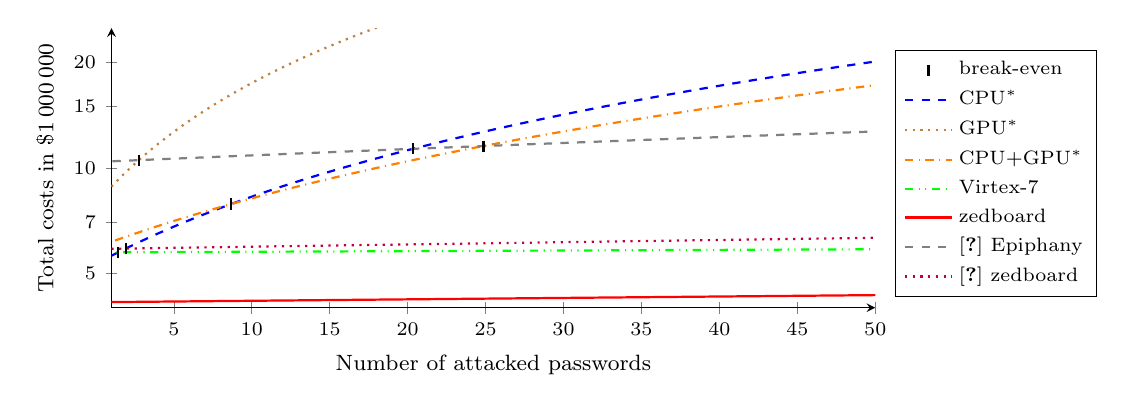
\begin{tikzpicture}
	\pgfplotsset{
		height=3.55cm, width=.8\textwidth,
		scale only axis,
		legend columns=1,
		legend style={at={(1,0.5)},
					  xshift=0.25cm,
					  yshift=1.5cm,
					  anchor=north west,
					  nodes=right,
					  font=\scriptsize,
					 },
		every axis plot post/.append style={
			mark=none,
			domain=0:50,
			samples=100,
			thick},
		}
	\begin{axis}[
		scatter/classes={a={mark=|,black}},
		axis y line=left,
		axis x line=bottom,
		x tick label style={font=\scriptsize},
		y tick label style={font=\scriptsize},
		xlabel style={font=\footnotesize},
		xlabel=Number of attacked passwords,
		ylabel style={font=\footnotesize},
		ylabel=Total costs in \$1\,000\,000,
		%xtick={25, 50, 75, 100, 125, 150, 175},
		xmin=1, xmax=50,
		ytick={5000000, 7000000, 10000000, 15000000, 20000000},
		yticklabels={$5$, $7$, $10$, $15$, $20$},
		ymin=4000000, ymax=25000000,
		ymode=log,
		cycle list name=linestyles*
		]
		\addplot+[color=black,only marks,scatter,scatter src=explicit symbolic] coordinates{
			(2.75, 10525390.42) [a]
			(1.91, 5895676.33) [a]
			(20.33, 11335789.16) [a]
			(1.43, 5752687.56) [a]
			(24.86, 11544263.66) [a]
			(8.69, 7897759.68) [a]
			(1017.0, 8177871.0) [a]
		};
		\addplot+[color=blue]{5330652+295327*x}; %CPU
		\addplot+[color=brown]{7896960+955217*x}; %GPU
		\addplot+[color=orange]{5936853+225588*x}; %CPU+GPU
		\addplot+[color=green]{5749275+2388*x}; %Virtex7
		\addplot+[color=red]{4146681+3963*x}; %zedboard
		\addplot+[color=gray]{10398561+46092*x}; %Epiphany
		\addplot+[color=purple]{5878532+8961*x}; %OWzb
		\legend{
			break-even, CPU$^*$, GPU$^*$, CPU+GPU$^*$,
			Virtex-7, zedboard,
			\cite{WOOT/Malvoni14}~Epiphany, \cite{WOOT/Malvoni14}~zedboard
			}
	\end{axis}
	\end{tikzpicture}
	\caption{Total costs in \textit{millions USD} for attacking $n$ passwords of length 8 from a set of
	62 characters, with logarithmic scale. Each attack finishes within
	\textit{one month}. Both the acquisition costs for enough devices and the total power costs
	where considered.}
	\label{fig:costs_for_password_cracking}
	\end{minipage}%
	\hspace{2.cm}
	\begin{minipage}[b]{0.45\textwidth} \centering
	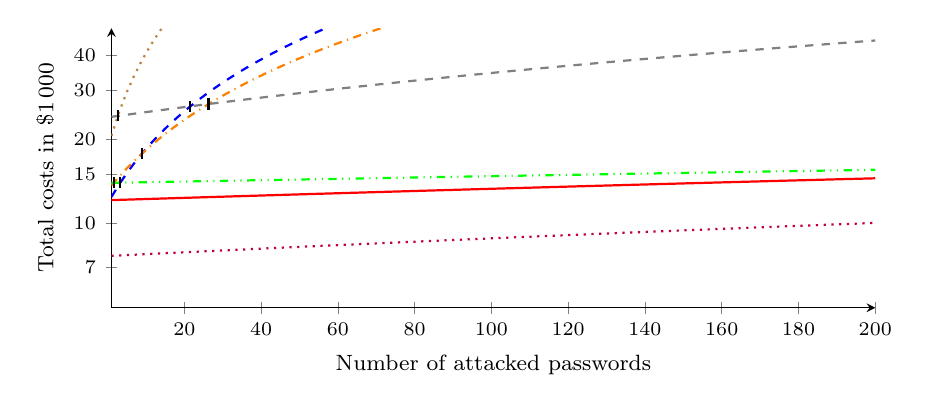
\begin{tikzpicture}
	\pgfplotsset{
		height=3.55cm, width=.8\textwidth,
		scale only axis,
		legend columns=3,
		legend style={column sep=1ex,
					  at={(0,0)},
					  xshift=0.25cm,
					  yshift=-1.0cm,
					  anchor=north west,
					  nodes=right,
					  font=\scriptsize
					 },
		every axis plot post/.append style={
			mark=none,
			domain=1:200,
			samples=100,
			thick},
		}
	\begin{axis}[
		scatter/classes={a={mark=|,black}},
		axis y line=left,
		axis x line=bottom,
		x tick label style={font=\scriptsize},
		y tick label style={font=\scriptsize},
		xlabel style={font=\footnotesize},
		xlabel=Number of attacked passwords,
		ylabel style={font=\footnotesize},
		ylabel=Total costs in \$1\,000,
		%xtick={25, 50, 75, 100, 125, 150, 175},
		xmin=1, xmax=200,
		ytick={7000, 10000, 15000, 20000, 30000, 40000},
		yticklabels={$7$, $10$, $15$, $20$, $30$, $40$},
		ymin=5000, ymax=50000,
		ymode=log,
		cycle list name=linestyles*
		]
		\addplot+[color=black,only marks,scatter,scatter src=explicit symbolic] coordinates{
			(0.5, 12128.04) [a]
			(1.57, 13992.59) [a]
			(26.3, 26776.98) [a]
			(2.64, 24268.6) [a]
			(1581.0, 26628.0) [a]
			(464.0, 17692.0) [a]
			(21.55, 26273.62) [a]
			(3.3, 14006.39) [a]
			(8.96, 17811.99) [a]
		};
		\addplot+[color=blue]{11790+672*x}; % CPU
		\addplot+[color=brown]{18360+2240*x}; % GPU
		\addplot+[color=orange]{13179+517*x}; % CPU+GPU
		\addplot+[color=green]{13980+8*x}; % Virtex7
		\addplot+[color=red]{12122+12*x}; % zedboard
		\addplot+[color=gray]{23989+106*x}; % Epiphany
		\addplot+[color=purple]{7656+12*x}; % OWzb
	\end{axis}
	\end{tikzpicture}
	\caption{Total costs in \textit{thousands USD} for attacking $n$ passwords of length 8 from a set of
	62 characters using a cost parameter of 12 (which is commonly recommended),
	with logarithmic scale. Each attack finishes within \textit{one day}, with a
	\textit{dictionary attack} where 65\% are covered ($\text{4} \cdot \text{10}^\text{9}$ Tests).}
	\label{fig:costs_for_dict_attack}
	\end{minipage}%
\end{figure*}

Table~\ref{tab:results_different_plattforms} compares the different
implementation platforms for cost parameter of 5 and 12. For better
comparison, Figure~\ref{fig:implementation_comparison} shows the performance and
efficiency graphically only for the first case.
%
Our zedboard implementation outperforms the previous implementation from
\cite{WOOT/Malvoni14} by a factor of 1.42, computing 6511~pps at a measured
power consumption of only 4.2W compared to 6.7W of the previous
implementation. Thus, this implementation yields also a better power efficiency
of 1550 pps per watt, which is more than twice as efficient as the previous
implementation. The CPU attack on a Xeon computes 5\% less pps, at a
significantly higher power consumption. Even considering only the power
consumption of the CPU itself of 80W, the efficiency of the zedboard is still
about 20 times higher. The estimated Virtex-7 design shows that the
high-performance board is a decent alternative to the zedboard: it outperforms
all other platforms with 51437 pps and has a very high power-efficiency rating.
The drawback is the high price of \$3495 for the development board.

To analyze the full costs of an attack, including the necessary power
consumption (at the price of 10.08 cents per kWh\footnote{Taken from the
\enquote{Independent Statistics \& Analysis U.S. Energy Information
Administration}, average retail price of electricity United States all sectors.
\url{http://www.eia.gov/electricity/data/browser}}), we consider two different
scenarios. The first uses the fairly low cost parameter of 5 for a simple
brute-force attack on passwords of length 8 with 62 different characters and
requires the runtime to be at most 1 month. We chose the considerably low cost
parameter for comparison with the related work, as it is typically used for
bcrypt benchmarks. However, this value is insecure for practical
applications, where a common choice seems to be 12, which is also used in
the related work. Thus, we use this more reasonable parameter in the second setting.
Here, the adversary uses more sophisticated attacks and aims for a reduction of
the number of necessary password guesses and for a reduced runtime of one day
per cracked password: We consider an adversary with access to meaningful,
target-specific, custom dictionaries -- for example generated through social
engineering -- and derivation rules.
%
In~\cite{PBKDEvalutation}, the authors trained on a random subset of 90\% from
the leaked RockYou passwords to attack the remaining 10\% and estimated that
$\text{4} \cdot \text{10}^\text{9}$ guesses are needed for about 67\% chance of
success, which we use as a basis for the computational power.

Figure~\ref{fig:costs_for_password_cracking} shows the costs of running
brute-force attacks in the first scenario. To achieve the requested amount of
password tests in one month, we need 13564 single CPUs, 43872 GPUs,
10361 CPUs + GPUs, 12999 zedboards or 1645 Virtex-7 boards. The figure
shows the total costs considering acquisition costs (fixed cost) and the power
consumption. It reveals the infeasibility of CPUs for attacking password hashes,
and even more clearly the efficiency of special-purpose devices. Even
high-performance FPGAs like the Virtex-7 are more profitable after only a few
password cracks, than a combination of CPU and GPU.

Figure~\ref{fig:costs_for_dict_attack} shows the costs of attacking multiple
passwords in the second scenario. Here, we need 30 CPUs, 102 GPUs, 23
CPUs + GPUs, 38 zedboards or 4 Virtex-7 boards.
%Even though we consider a much higher cost parameter and require a runtime of
%one day per password, the attack is still cheaper due to the smarter derivation
%of password candidates.
With the higher cost parameter our current zedboard implementation does not yield
similar good results and thus \cite{WOOT/Malvoni14} implementation is currently
better suited for this attack when mounted on a zedboard. With the higher cost
parameter, their implementation can conceal an interface bottleneck coming from
the initialization of the bcrypt cores. As our implementation does not suffer from
this bottleneck, we can run several cores on a bigger FPGA without negative
consequences. Please note that the Virtex-7, after amortizing its acquisition costs,
outperforms every other platform (reaching the break-even point with
\cite{WOOT/Malvoni14} zedboard after attacking about 1500 passwords).

%Comparing CPUs with low-power targets like the zedboard leads to the same result
%as before -- power efficiency has a great impact on overall attack costs.
%Therefore, FPGA platforms are better suited for attacking passwords and a
%successful attacker does not have to spend more than \$10000 for cracking
%passwords.

%!TEX root = main.tex

\section{Conclusion and Future Work}
\label{sec:conclusion}
In this paper, we presented a highly optimized bcrypt implementation on FPGAs.
We use a quad-core structure to achieve an optimal resource utilization and gain
a speed-up of 42\% and -- due to lower power consumption -- increased
power-efficiency by 127\% compared to the previous results on the same device.
In the design we presented, the critical path is still within the Blowfish core,
resulting in a moderate clock-frequency of 100 MHz. An idea to improve this is to
pipeline the encryption within a quad-core, interleaving the computations of the
core. This may shorten the critical path further, allowing higher clock
frequencies and more parallel bcrypt cores due to shared resources.

We showed that it is possible to utilize the remaining fabric area to
implement a small on-chip password generation, which is adaptable and may be
combined with a dictionary attack, \eg for prefix and suffix modifications.
These possibilities should be evaluated and further analyzed, as the password
generation has a high impact on the success rate. Even more importantly, using
only off-chip password generation, \ie by using a CPU to generate passwords and transfer
them to the FPGA, introduces two potential bottlenecks: the software
implementation itself and the data bus. With the combination of off-chip
creation and on-chip modification, it should be possible to reduce the risk of these
bottlenecks even in large and highly parallelized clusters: We can use the password
generator construction for simple mangling rules and relax the interface or
dedicate several cores to brute-force attacks, while others work on a dictionary.
This leads to more possible trade-offs in terms of interface speed vs. area
consumption.

In our attack scenarios, we considered modern representatives of CPUs as well as
GPUs and benchmarked the (ocl)Hashcat bcrypt implementation on these platforms.
We compared the total costs of low-power and high-performance devices in two
scenarios: simple brute-force with a fixed runtime of 1 month (cost 5) and an
advanced attack with a timeframe of 1 day (cost 12). In both cases, the high
power consumption of CPUs and GPUs renders large-scale attacks infeasible, as
our FPGA implementation not only outperforms these devices but also requires
significantly less power. 

Interestingly, in combination with improved methods to derive suitable password
candidates, the overall costs when using a fast and power-efficient FPGA
implementation are not as high as expected for reasonable parameters.  As a
result, we should evaluate and adjust the parameters used in practice to
withstand the advances in technology and intelligent password generation.


\bibliographystyle{IEEEtran}
\bibliography{bcrypt}

\end{document}
